\chapter{ROC curves}
This chapter is based on Ref.\cite{wiki-roc}.

ROC stands for
{\bf  Receiver Operating Characteristic}.
ROC curves are used in binary
classification (BC).

To do BC, we are given the value
$x\in\RR$
for an individual. From this, 
we want to decide
whether that
individual 
has $a=T=True$
or $a=F=False$.
The decision will
depend on the
value
assigned to
a {\bf threshold parameter $\tau\in \RR$}.


\begin{figure}[h!]
$$\xymatrix{
\rvx&\rva\ar[l]
}$$
\caption{bnet for 
BC.}
\label{fig-hyp-bnet}
\end{figure}
Fig.\ref{fig-hyp-bnet}
shows the bnet used for BC.


\begin{figure}[h!]
\centering
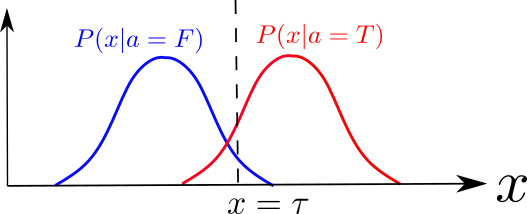
\includegraphics[width=3in]
{roc/bell-curves.png}
\caption{$x$-distribution for
two hypotheses $a=F,T$. } 
\label{fig-bell-curves}
\end{figure}
Fig.\ref{fig-bell-curves}
is a 
plot
of $P(x|a)$, the TPM 
for node $\rvx$
of the bnet in Fig.\ref{fig-hyp-bnet}.


\begin{figure}[h!]
\centering
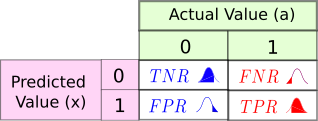
\includegraphics[width=3in]
{roc/confusion-mat.png}
\caption{The confusion matrix 
$P(b|a)$
for BC.} 
\label{fig-confusion-mat}
\end{figure}

Whereas $a$
is binary, $x$
is continuous. 
But we can replace
$x$ by a binary variable

\beq
b=\indi(x>\tau)
\;.
\eeq
$P(b|a)$
for $b\in\bool$
and $a\in \{F,T\}$
is called the
{\bf confusion matrix}
or {\bf contingency table}
for BC.
The confusion
matrix can be
calculated from
the TPM $P(x|a)$.
Fig.\ref{fig-confusion-mat}
illustrates the
confusion matrix
$P(b|a)$
for BC.
In that
figure,
the rates $R$
are defined as
follows.

\begin{itemize}
\item {\color{blue}\bf False Positive rate}
\beqa
\color{blue}
R_{FP}(\tau)&=&
P(x>\tau|a=F)= \int_{x>\tau}dx\;P(x|a=F)
\eeqa
In Hypothesis Testing,
$R_{FP}$ is also called the {\bf p-value that $\rvx>\tau$
assuming curve $F$ is the
null hypothesis}.

\item{\color{blue}\bf False Negative rate}
\beqa
\color{blue}
R_{FN}(\tau)&=&1-R_{FP}(\tau)
\\
&=&
 P(x<\tau|a=F)= \int_{x<\tau}dx\;P(x|a=F)
\eeqa

\item{\color{red}\bf True Positive  rate}
\beqa
\color{red}
R_{TP}(\tau)&=& 
P(x>\tau|a=T)=\int_{x>\tau}dx\;P(x|a=T)
\eeqa
In Hypothesis Testing,
$R_{TP}$ is called the {\bf p-value that $\rvx>\tau$
assuming curve $T$ is the
null hypothesis}.

\item {\color{red}\bf True Negative rate}
\beqa
\color{red}
R_{TN}(\tau)&=& 1-R_{TP}(\tau)
\\
&=& P(x<\tau|a=T)= \int_{x<\tau}dx\;P(x|a=T)
\eeqa
\end{itemize}

\begin{figure}[h!]
\centering
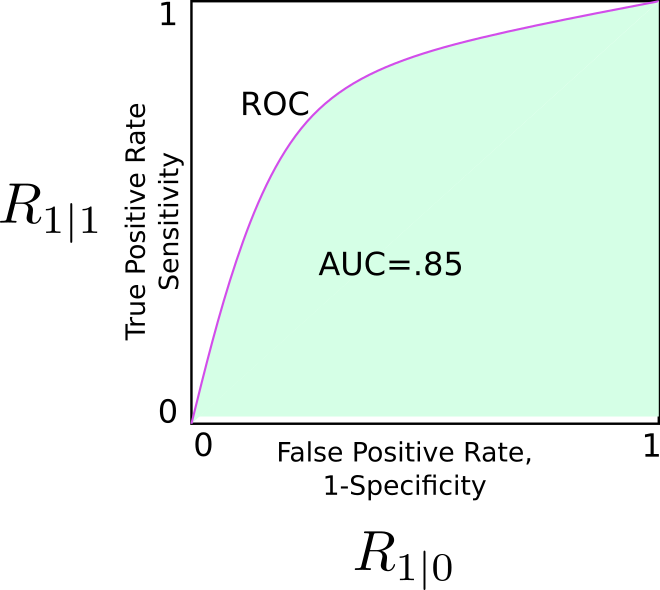
\includegraphics[width=2in]
{roc/roc-auc.png}
\caption{Example of ROC.
Green shaded
 area is the AUC of the ROC.} 
\label{fig-roc-auc}
\end{figure}

\begin{figure}[h!]
\centering
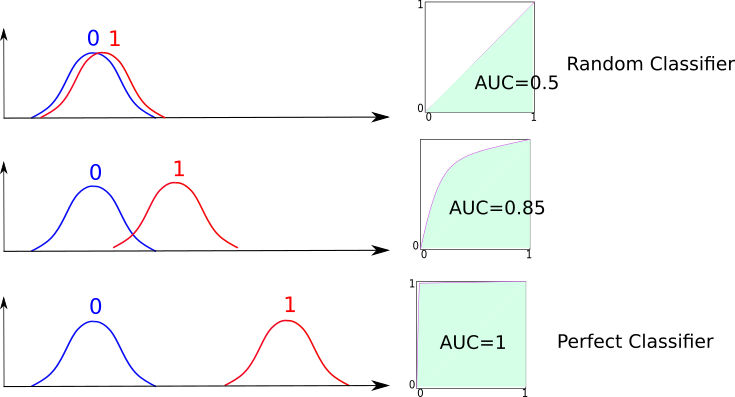
\includegraphics[width=4in]
{roc/roc-panels.png}
\caption{
ROC curves for
3 different separations
between the T and F 
x-distributions.} 
\label{fig-roc-panels}
\end{figure}



The {\bf Receiver Operating Characteristic 
(ROC)} is a
parametric plot with  $X=R_{FP}(\tau)$
and $Y=R_{TP}(\tau)$
and $\tau\in\RR$.
The {\bf Area Under the Curve (AUC)}
is the area under the ROC.
Fig.\ref{fig-roc-auc}
shows an example of a ROC and AUC.

As shown in Fig.\ref{fig-roc-panels},
AUC ranges from $0.5$ for
a random classifier to $1$ 
for a perfect classifier.
Note that

\beqa
AUC &=&\int_{x=0}^1 d\tau\;\;
R_{TP}(\tau)
\frac{dR_{FP}(\tau)}{d\tau}
\\
&=&
\int_{\infty}^{-\infty} d\tau\;\;
\left\{\int_{-\infty}^\infty dx\;\;
\indi(x>\tau) P(x|a=T)\right\}
(-1)P(x=\tau|a=F)
\\
&=&
\int_{-\infty}^\infty dx'\;\;
\int_{-\infty}^\infty dx\;\;
\indi(x>x') P(x|a=T)
P(x'|a=F)
\;.
\eeqa

